% Appendix: A Related Works, B Proof, C Implementation Details, D Additional Experiments, E Simulation Study.
\section{Related Works} \label{apdx:related-works}

\subsection{Test-Time Normalization}
Re-estimating BN statistics on target data is a simple and widely adopted response to covariate shift.
AdaBN \cite{AdaBN} replaces the source statistics by target-domain statistics for domain adaptation, and prediction-time BN \cite{PredictionBN} and the covariate shift adaptation of \citet{BN-Adapt} recompute them on each test batch, \citet{BN-Adapt} with a pseudo sample size $N$ that mixes in the source statistics.
$\alpha$-BN \cite{AlphaBN} mixes the two with a constant weight, DUA \cite{DUA} updates them with a decaying momentum over the stream, TTN \cite{TTN} learns a per-layer interpolation in a post-training phase on source data, and UnMix-TNS \cite{UnMix-TNS} and NOTE \cite{NOTE} handle test streams whose labels are correlated in time.
While effective, such rules fix how much they trust a test batch in advance (by a hyperparameter, a schedule or weights learned on source data), and they remain exposed to stale source statistics under large shifts and to noisy batch statistics under small batches.

\subsection{Test-Time Adaptation with Gradient Updates}
A second line updates model parameters on the test data.
TENT \cite{TENT} minimizes the prediction entropy with respect to the BN affine parameters, SAR \cite{SAR} reports that BN makes such updates unstable for small batches and filters samples with large gradients, and DELTA \cite{DELTA} renormalizes test-time BN statistics and reweights classes to remove biased updates.
These methods all rely on some estimate of the normalization statistics, and Section~\ref{sec:extension} shows that the choice of this estimate changes their error.
However, how to set the statistics of each batch without any hyperparameter remains largely underexplored in this line.

\subsection{Shrinkage Estimation in Normalization Layers}
The James--Stein estimator \cite{James-Stein} improves the sample mean of three or more Gaussian means by shrinking it toward a fixed point, and the empirical Bayes view of \citet{Efron-Morris} explains the shrinkage factor as an estimate of the signal-to-noise ratio.
Recent work applies Stein shrinkage inside normalization layers during training: \citet{JS-Norm} shrink the batch means and variances of each layer toward their cross-channel average, and \citet{Stein-BN-Adv} prove that such shrinkage dominates the sample estimates under sub-Gaussian adversarial perturbations.
These methods shrink toward a centre computed from the same batch, during training, to reduce noise rather than to correct a shift.
To address these gaps, we propose SourceStein, which shrinks the test batch statistics toward the source statistics at test time, so that one closed-form weight per layer is adaptive and stable: it follows the shift when the batch contains evidence for it and keeps the source statistics otherwise.

\clearpage
\section{Proof of Proposition~\ref{prop:risk}} \label{apdx:proof}
\textbf{Setup.} Our goal is to bound the risk of Equation~\ref{eq:risk} at the Stein weight.
Let $\mathbf{z} = \sqrt{n}\,\boldsymbol{\Sigma}^{-1/2}\hat{\boldsymbol{\mu}}$, $\boldsymbol{\theta} = \sqrt{n}\,\boldsymbol{\Sigma}^{-1/2}\boldsymbol{\mu}^{\text{tgt}}$ and $\mathbf{a} = \sqrt{n}\,\boldsymbol{\Sigma}^{-1/2}\boldsymbol{\mu}^{\text{src}}$.
Under the assumption $\hat{\boldsymbol{\mu}} \sim \mathcal{N}(\boldsymbol{\mu}^{\text{tgt}}, \boldsymbol{\Sigma}/n)$, we have $\mathbf{z} \sim \mathcal{N}(\boldsymbol{\theta}, \mathbf{I}_C)$.
For any weight $\lambda$, possibly depending on $\mathbf{z}$, the whitening is linear, so:
\begin{equation*}
n\,\|\boldsymbol{\mu}(\lambda) - \boldsymbol{\mu}^{\text{tgt}}\|^2_{\boldsymbol{\Sigma}^{-1}} = \|\mathbf{a} + \lambda(\mathbf{z} - \mathbf{a}) - \boldsymbol{\theta}\|^2,
\end{equation*}
and the shift score of Equation~\ref{eq:shift-score} is $S = \|\mathbf{z} - \mathbf{a}\|^2$.

\textbf{Risk of the Stein weight.} With $\lambda = 1 - (C-2)/S$, the estimator $\mathbf{a} + \lambda(\mathbf{z} - \mathbf{a})$ is the James--Stein estimator with target $\mathbf{a}$, whose risk is $C - (C-2)^2\,\mathbb{E}[1/S]$ by Lemma~\ref{lemma:james-stein}; the positive part $\hat{\lambda}$ of Equation~\ref{eq:stein-weight} has no larger risk \cite{Efron-Morris}.
Since $S$ follows a noncentral $\chi^2$ distribution with $C$ degrees of freedom and noncentrality $\|\boldsymbol{\theta} - \mathbf{a}\|^2 = \Delta$, we have $\mathbb{E}[S] = C + \Delta$.
Since the function $x \mapsto 1/x$ is convex on $(0, \infty)$, Jensen's inequality yields $\mathbb{E}[1/S] \ge 1/(C + \Delta)$, which is finite for $C \ge 3$.
We conclude:
\begin{equation*}
R(\hat{\lambda}) \le C - \frac{(C-2)^2}{C + \Delta} < C = R(1),
\end{equation*}
where $R(1) = \mathbb{E}\|\mathbf{z} - \boldsymbol{\theta}\|^2 = C$ is the risk of TBN.

\textbf{Excess over the oracle weight.} Subtracting $R(\lambda^{\star}) = C\Delta/(C + \Delta)$ from Equation~\ref{eq:oracle}:
\begin{equation*}
R(\hat{\lambda}) - R(\lambda^{\star}) \le \frac{C(C + \Delta) - (C-2)^2 - C\Delta}{C + \Delta} = \frac{4(C-1)}{C + \Delta} \le \frac{4(C-1)}{C} < 4.
\end{equation*}
Therefore, the bound holds for each shift $\boldsymbol{\delta}$ and batch size $n$, and the excess is largest without any shift ($\Delta = 0$), where the oracle keeps the source mean exactly. \hfill$\square$

\clearpage
\section{Implementation Details} \label{apdx:impl-details}
All experiments run on one CPU machine (15 cores, no GPU) with PyTorch\footnote{\url{https://pytorch.org}} 2.8 and NumPy; the code that produced each number is part of the supplementary material.

\textbf{Source models.} CNN-8 stacks three stages of two $3{\times}3$ convolutions with 32, 64 and 128 channels, each followed by BN and ReLU, with max pooling between stages, global average pooling and a linear head. ResNet-14 is the CIFAR residual network of \citet{ResNet} with two basic blocks per stage (widths 16, 32, 64), 15 BN layers in total. Table~\ref{tab:hyper} reports the training recipe; training took 11.6 min (CNN-8) and 11.9 min (ResNet-14) of wall-clock time on 7 threads each.

\begin{table}[ht]
\centering
\caption{Training and evaluation settings.}
\label{tab:hyper}
\begin{tabular}{l|c}
\toprule
\textbf{Setting} & \textbf{Value} \\
\midrule
Optimizer & SGD, Nesterov momentum 0.9, weight decay $5 \times 10^{-4}$ \\
Learning rate & one-cycle schedule, peak 0.1, 15\% warm-up \\
Batch size / epochs & 128 / 8 (CNN-8), 5 (ResNet-14) \\
Augmentation & 4-pixel reflect padding + random crop, horizontal flip \\
Source images for $\boldsymbol{\tau}^2, \boldsymbol{\rho}^2$ & 5,000 random training images, no augmentation \\
Test images per corruption & 1,000 (fixed random subset per corruption) \\
Floor on the variance & $10^{-5}$ \\
TENT & Adam, learning rate $10^{-3}$, one step per batch, BN affine parameters only \\
\bottomrule
\end{tabular}
\end{table}

\textbf{Baselines.} TBN uses the biased batch variance over all $nHW$ positions. Prior-BN follows Equation~3 of \citet{BN-Adapt} for the mean and the variance. $\alpha$-BN follows \citet{AlphaBN} and mixes the means and the standard deviations with $\alpha = 0.9$. Oracle-$N$ selects, for each network and batch size, the best $N \in \{2, 4, 8, 16, 32, 64, 128, 256\}$ by the average error over the 15 corruptions; the selected values are $N = 4, 8, 8, 16, 16, 8, 64$ for ResNet-14 and $N = 2, 4, 4, 8, 4, 2, 2$ for CNN-8 at $n = 1, 2, 4, 8, 16, 64, 200$.

\textbf{Procedure.} The network applies Algorithm~\ref{alg:sourcestein} layer by layer in its forward pass, and each layer receives the features adapted by the layers before it.



\textbf{Data.} CIFAR-10-C \cite{CIFAR10-C} was downloaded from its official Zenodo record; we read only the severity-3 and severity-5 slices of the 15 standard corruptions. \textbf{Compute.} Besides training, the full evaluation of Table~\ref{tab:main-table} (all rules, ablations and all values of $N$, both severities) took 7.9 min (ResNet-14, 11 processes) and 12.2 min (CNN-8, 6 processes, partly in parallel), the TENT runs 4.8 and 3.7 min, and the simulation 2 s.

\clearpage
\section{Additional Experiments} \label{apdx:experiments}

\subsection{Results at Severity 3} \label{apdx:severity3}
Table~\ref{tab:apdx-sev3} repeats Table~\ref{tab:main-table} at the milder severity 3.
SourceStein has the lowest error from $n{=}2$ upward on both networks (TBN is 0.01 points lower at $n{=}64$ on CNN-8), while at $n{=}1$ the fixed weights of $\alpha$-BN and Prior-BN, which stay close to the source, are lower; under a mild shift, a single image contains little evidence and the shift bias of the source statistics is small.

\begin{table}[ht]
\centering
\renewcommand{\arraystretch}{0.9}
\caption{Error (\%) on CIFAR-10-C at severity 3, averaged over 15 corruptions. The best result in each column of a block is \textbf{bold}.}
\label{tab:apdx-sev3}
\begin{tabular}{cl|ccccccc}
\toprule
\textbf{Network} & \textbf{Method} & \textbf{1} & \textbf{2} & \textbf{4} & \textbf{8} & \textbf{16} & \textbf{64} & \textbf{200} \\
\midrule
\multirow{5}{*}{ResNet-14}
 & Source & 35.91 & 35.91 & 35.91 & 35.91 & 35.91 & 35.91 & 35.91 \\
 & TBN & 89.21 & 50.52 & 38.56 & 31.41 & 28.12 & 25.43 & 24.81 \\
 & Prior-BN & 33.35 & 31.03 & 29.09 & 27.55 & 26.87 & 25.25 & 24.79 \\
 & $\alpha$-BN & \textbf{31.88} & 31.04 & 30.35 & 29.79 & 29.50 & 29.12 & 29.19 \\
 & \cellcolor{oursrowblue}SourceStein & \cellcolor{oursrowblue}34.24 & \cellcolor{oursrowblue}\textbf{30.47} & \cellcolor{oursrowblue}\textbf{28.21} & \cellcolor{oursrowblue}\textbf{27.04} & \cellcolor{oursrowblue}\textbf{25.97} & \cellcolor{oursrowblue}\textbf{24.96} & \cellcolor{oursrowblue}\textbf{24.57} \\
\midrule\midrule
\multirow{5}{*}{CNN-8}
 & Source & 32.73 & 32.73 & 32.73 & 32.73 & 32.73 & 32.73 & 32.73 \\
 & TBN & 89.97 & 47.99 & 34.67 & 27.81 & 24.47 & \textbf{21.57} & 21.02 \\
 & Prior-BN & 30.69 & 28.68 & 26.51 & 24.49 & 23.25 & 21.71 & 20.99 \\
 & $\alpha$-BN & \textbf{29.53} & 28.73 & 28.43 & 28.13 & 27.82 & 27.70 & 27.61 \\
 & \cellcolor{oursrowblue}SourceStein & \cellcolor{oursrowblue}31.30 & \cellcolor{oursrowblue}\textbf{28.03} & \cellcolor{oursrowblue}\textbf{25.70} & \cellcolor{oursrowblue}\textbf{23.81} & \cellcolor{oursrowblue}\textbf{22.95} & \cellcolor{oursrowblue}21.58 & \cellcolor{oursrowblue}\textbf{20.91} \\
\bottomrule
\end{tabular}
\end{table}

\subsection{Per-Corruption Results} \label{apdx:per-corruption}
Table~\ref{tab:apdx-per-corruption} breaks down the error at $n{=}4$ by corruption.
SourceStein is the lowest of the five rules on 12 of the 15 corruptions for each network; its largest gain over the best other rule is on contrast for ResNet-14 (11.6 points) and on Gaussian noise for CNN-8 (9.0 points), and it is not the lowest on elastic transform and JPEG for either network, on glass blur for ResNet-14 and on pixelate for CNN-8.

\begin{table}[ht]
\centering
\renewcommand{\arraystretch}{0.9}
\caption{Error (\%) per corruption at severity 5 for test batches of $n{=}4$ images. The best result in each column of a block is \textbf{bold}.}
\label{tab:apdx-per-corruption}
\shrinktofit{\linewidth}{%
\begin{tabular}{cl|ccccccccccccccc}
\toprule
 & \textbf{Method} & \textbf{Gauss.} & \textbf{Shot} & \textbf{Impul.} & \textbf{Defoc.} & \textbf{Glass} & \textbf{Motion} & \textbf{Zoom} & \textbf{Snow} & \textbf{Frost} & \textbf{Fog} & \textbf{Brit.} & \textbf{Contr.} & \textbf{Elast.} & \textbf{Pixel.} & \textbf{JPEG} \\
\midrule
\multirow{5}{*}{\rotatebox{90}{ResNet-14}} & Source & 61.1 & 58.9 & 67.0 & 52.1 & 65.0 & 51.7 & 52.1 & 43.1 & 53.4 & 49.7 & 24.7 & 77.4 & 37.6 & 57.8 & 29.3 \\
 & TBN & 49.0 & 48.0 & 52.9 & 40.3 & 54.0 & 39.4 & 36.3 & 50.4 & 45.5 & 43.4 & 35.2 & 43.3 & 46.2 & 41.4 & 41.5 \\
 & Prior-BN & 44.1 & 40.2 & 51.1 & 34.1 & \textbf{53.4} & 33.9 & 35.4 & 40.7 & \textbf{37.9} & 35.3 & 24.2 & 46.8 & 35.3 & 39.8 & 28.5 \\
 & $\alpha$-BN & 50.2 & 45.4 & 57.6 & 39.3 & 58.4 & 39.2 & 38.4 & 40.6 & 42.2 & 38.5 & 23.6 & 60.7 & \textbf{34.5} & 49.0 & \textbf{28.3} \\
 & \cellcolor{oursrowblue}SourceStein & \cellcolor{oursrowblue}\textbf{40.4} & \cellcolor{oursrowblue}\textbf{38.3} & \cellcolor{oursrowblue}\textbf{48.2} & \cellcolor{oursrowblue}\textbf{29.7} & \cellcolor{oursrowblue}54.5 & \cellcolor{oursrowblue}\textbf{30.3} & \cellcolor{oursrowblue}\textbf{32.4} & \cellcolor{oursrowblue}\textbf{38.8} & \cellcolor{oursrowblue}\textbf{37.9} & \cellcolor{oursrowblue}\textbf{33.9} & \cellcolor{oursrowblue}\textbf{22.4} & \cellcolor{oursrowblue}\textbf{31.7} & \cellcolor{oursrowblue}36.2 & \cellcolor{oursrowblue}\textbf{39.1} & \cellcolor{oursrowblue}29.7 \\
\midrule\midrule
\multirow{5}{*}{\rotatebox{90}{CNN-8}} & Source & 65.3 & 58.8 & 67.6 & 52.0 & 61.8 & 44.2 & 46.2 & 42.3 & 51.3 & 44.5 & 19.8 & 78.3 & 33.3 & 57.4 & 27.3 \\
 & TBN & 48.6 & 46.1 & 53.7 & 35.4 & 53.4 & 36.8 & 34.6 & 44.3 & 42.4 & 39.8 & 29.6 & 36.9 & 39.7 & \textbf{38.8} & 39.9 \\
 & Prior-BN & 48.4 & 43.2 & 54.0 & 33.6 & 52.9 & 31.4 & 34.1 & 36.8 & 37.6 & 33.8 & 17.0 & 64.9 & \textbf{29.9} & 42.3 & 27.8 \\
 & $\alpha$-BN & 54.3 & 49.9 & 59.9 & 40.6 & 57.0 & 35.5 & 38.7 & 37.5 & 41.5 & 35.9 & 18.1 & 71.5 & 30.6 & 50.1 & \textbf{27.0} \\
 & \cellcolor{oursrowblue}SourceStein & \cellcolor{oursrowblue}\textbf{39.4} & \cellcolor{oursrowblue}\textbf{35.5} & \cellcolor{oursrowblue}\textbf{50.2} & \cellcolor{oursrowblue}\textbf{29.2} & \cellcolor{oursrowblue}\textbf{52.1} & \cellcolor{oursrowblue}\textbf{28.6} & \cellcolor{oursrowblue}\textbf{31.0} & \cellcolor{oursrowblue}\textbf{35.2} & \cellcolor{oursrowblue}\textbf{36.7} & \cellcolor{oursrowblue}\textbf{29.9} & \cellcolor{oursrowblue}\textbf{16.6} & \cellcolor{oursrowblue}\textbf{35.6} & \cellcolor{oursrowblue}30.5 & \cellcolor{oursrowblue}41.7 & \cellcolor{oursrowblue}27.5 \\
\bottomrule
\end{tabular}}
\end{table}

\clearpage
\section{Simulation Study} \label{apdx:synthetic}
The simulation draws $C{=}64$ per-sample means with unit noise per channel, shifts the target mean from the source mean in a random direction of a given size, and averages the risk of Equation~\ref{eq:risk} (divided by $C$) over 4,000 batches per setting; SourceStein uses the source noise level, as in the networks.
Figure~\ref{fig:apdx-synthetic} shows three batch sizes under the Gaussian model and three departures from it at $n{=}4$.
With Student-$t$ noise of three degrees of freedom, SourceStein remains below TBN at each shift and exceeds the oracle by at most 0.114 per channel.
When the true noise is 0.7 times the stored level, SourceStein shrinks too much and exceeds TBN at 6 of the 14 shift sizes; when it is 1.4 times larger, SourceStein stays below TBN but keeps a floor of about 0.5 at zero shift.
These cases mark the assumption of Proposition~\ref{prop:risk} that matters in practice: the noise level must be measured on data whose between-sample spread resembles that of the test data.

\begin{figure}[ht]
    \centering
    \begin{subfigure}[t]{0.32\columnwidth}
        \centering
        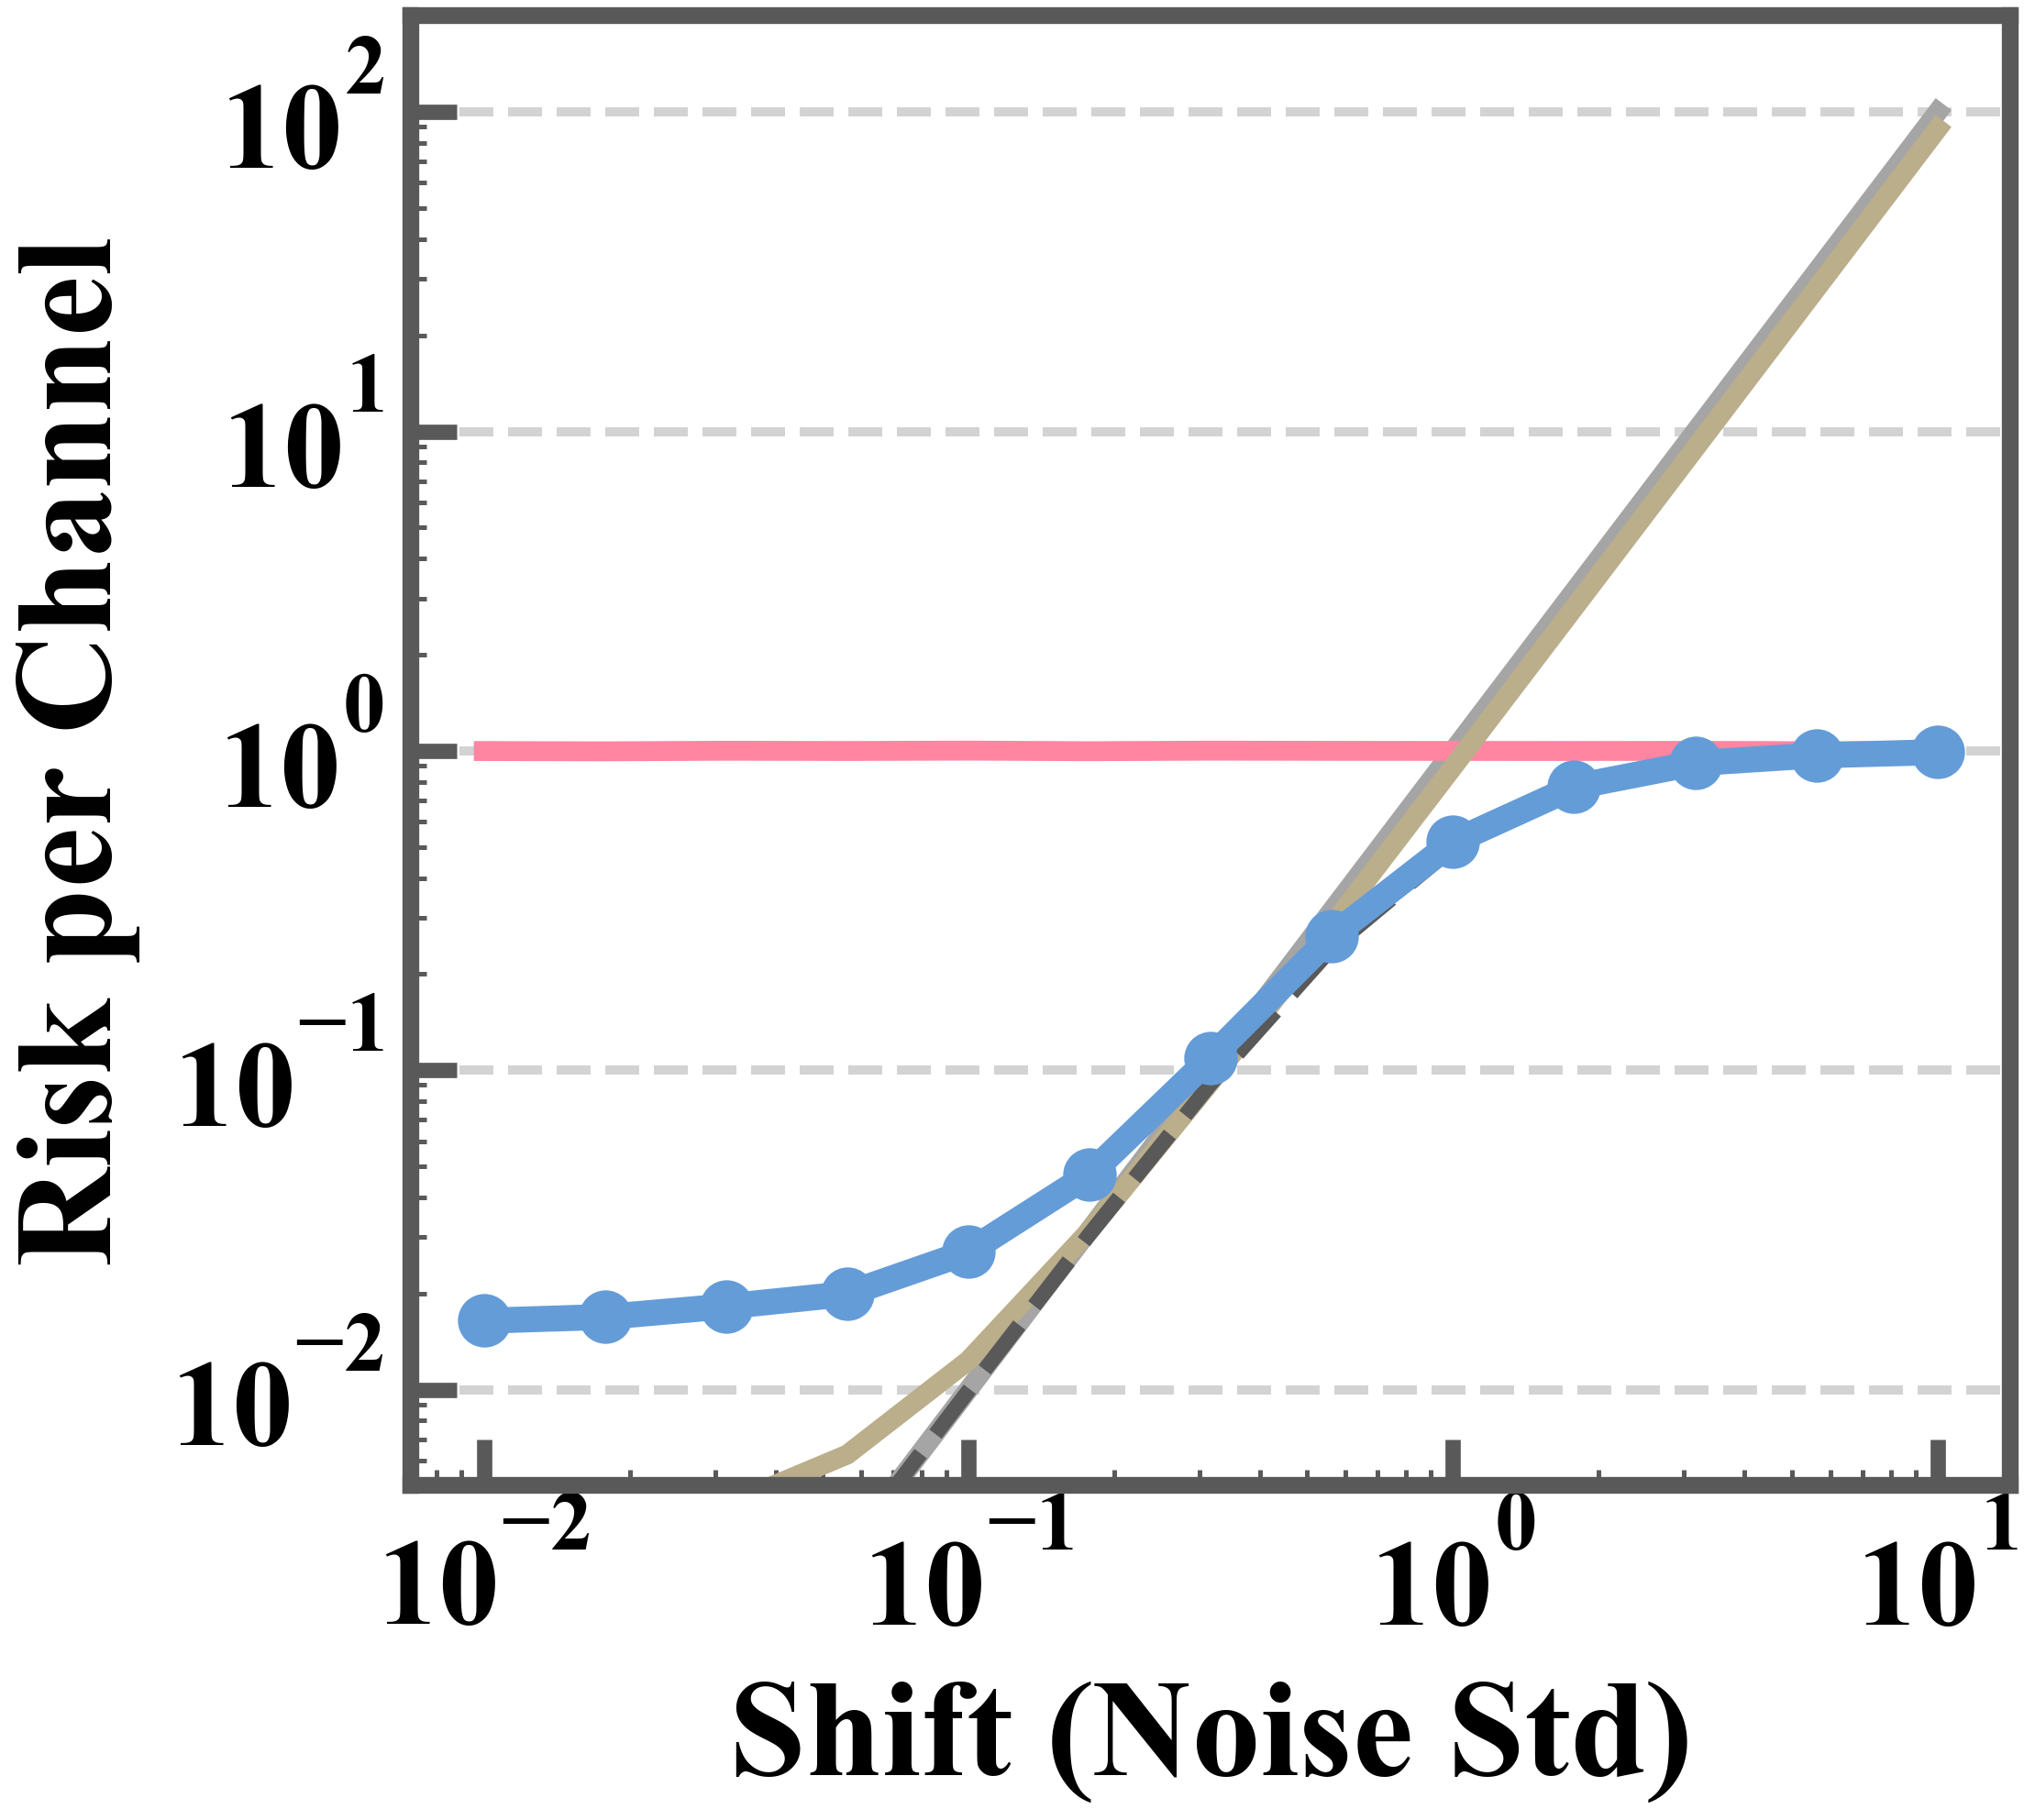
\includegraphics[width=\linewidth]{figures/exp/synthetic/risk_n1_gauss_s1p0.png}
        \caption{Gaussian, $n{=}1$.}
    \end{subfigure}\hfill
    \begin{subfigure}[t]{0.32\columnwidth}
        \centering
        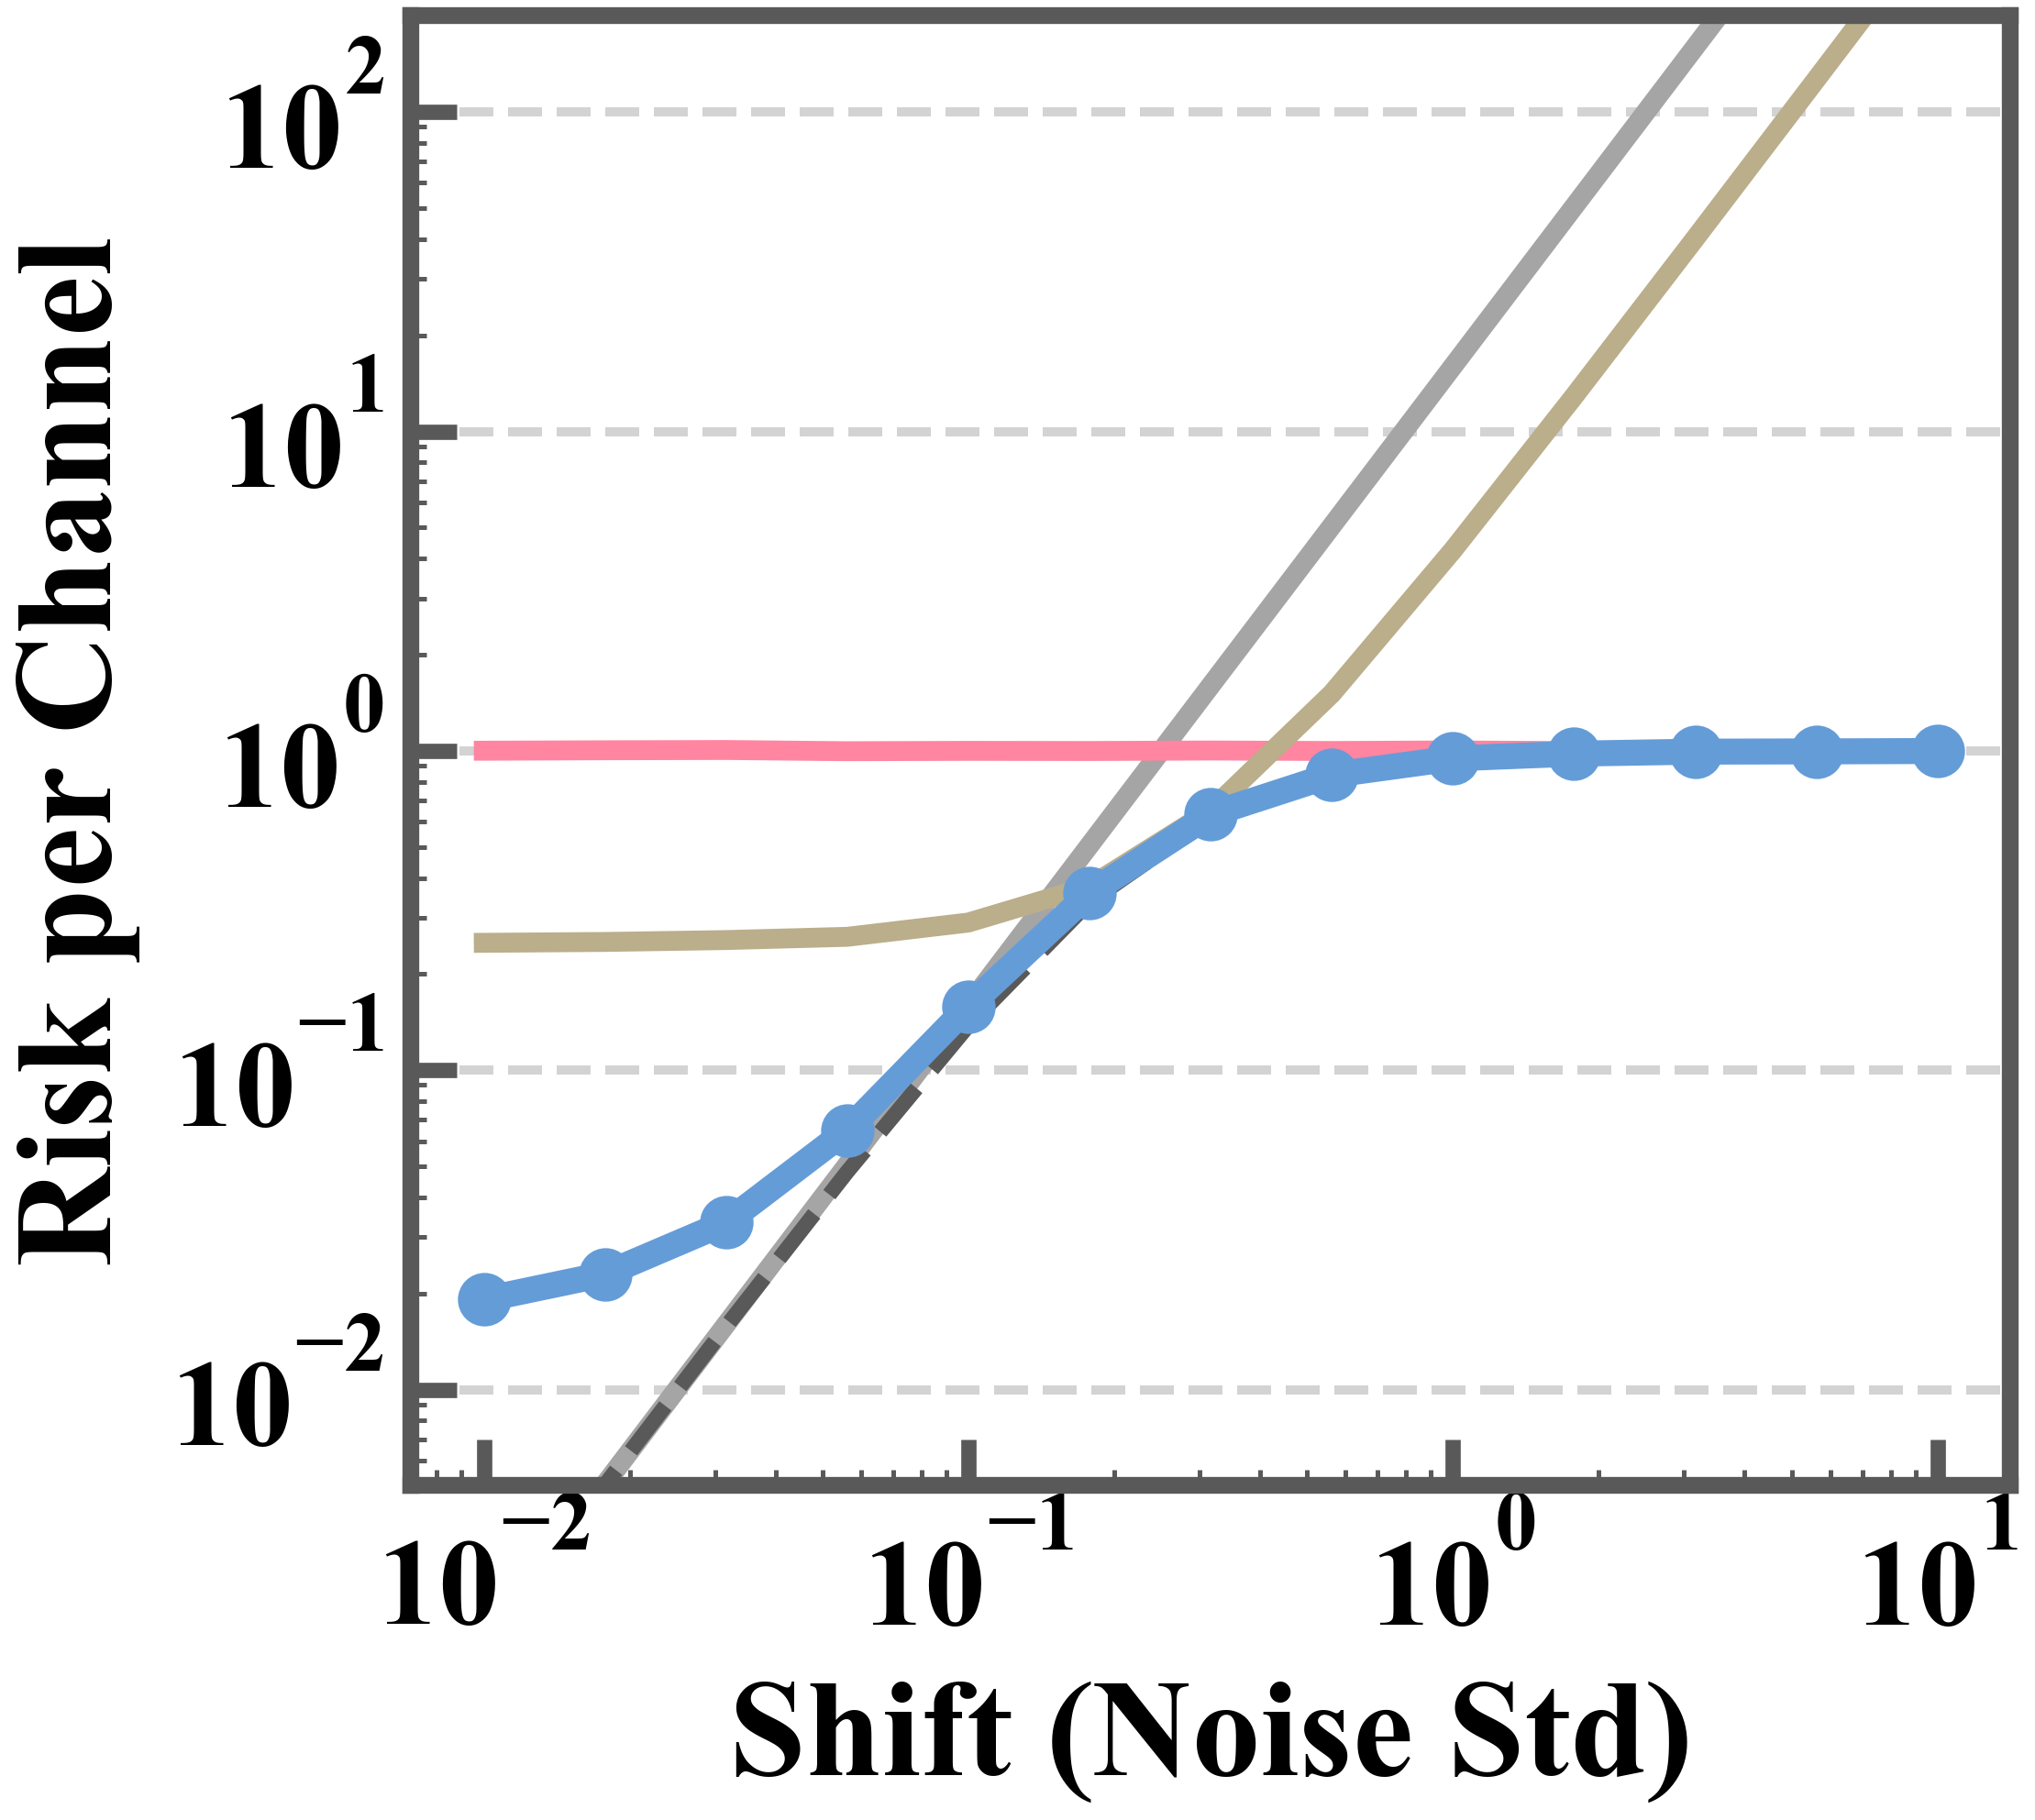
\includegraphics[width=\linewidth]{figures/exp/synthetic/risk_n16_gauss_s1p0.png}
        \caption{Gaussian, $n{=}16$.}
    \end{subfigure}\hfill
    \begin{subfigure}[t]{0.32\columnwidth}
        \centering
        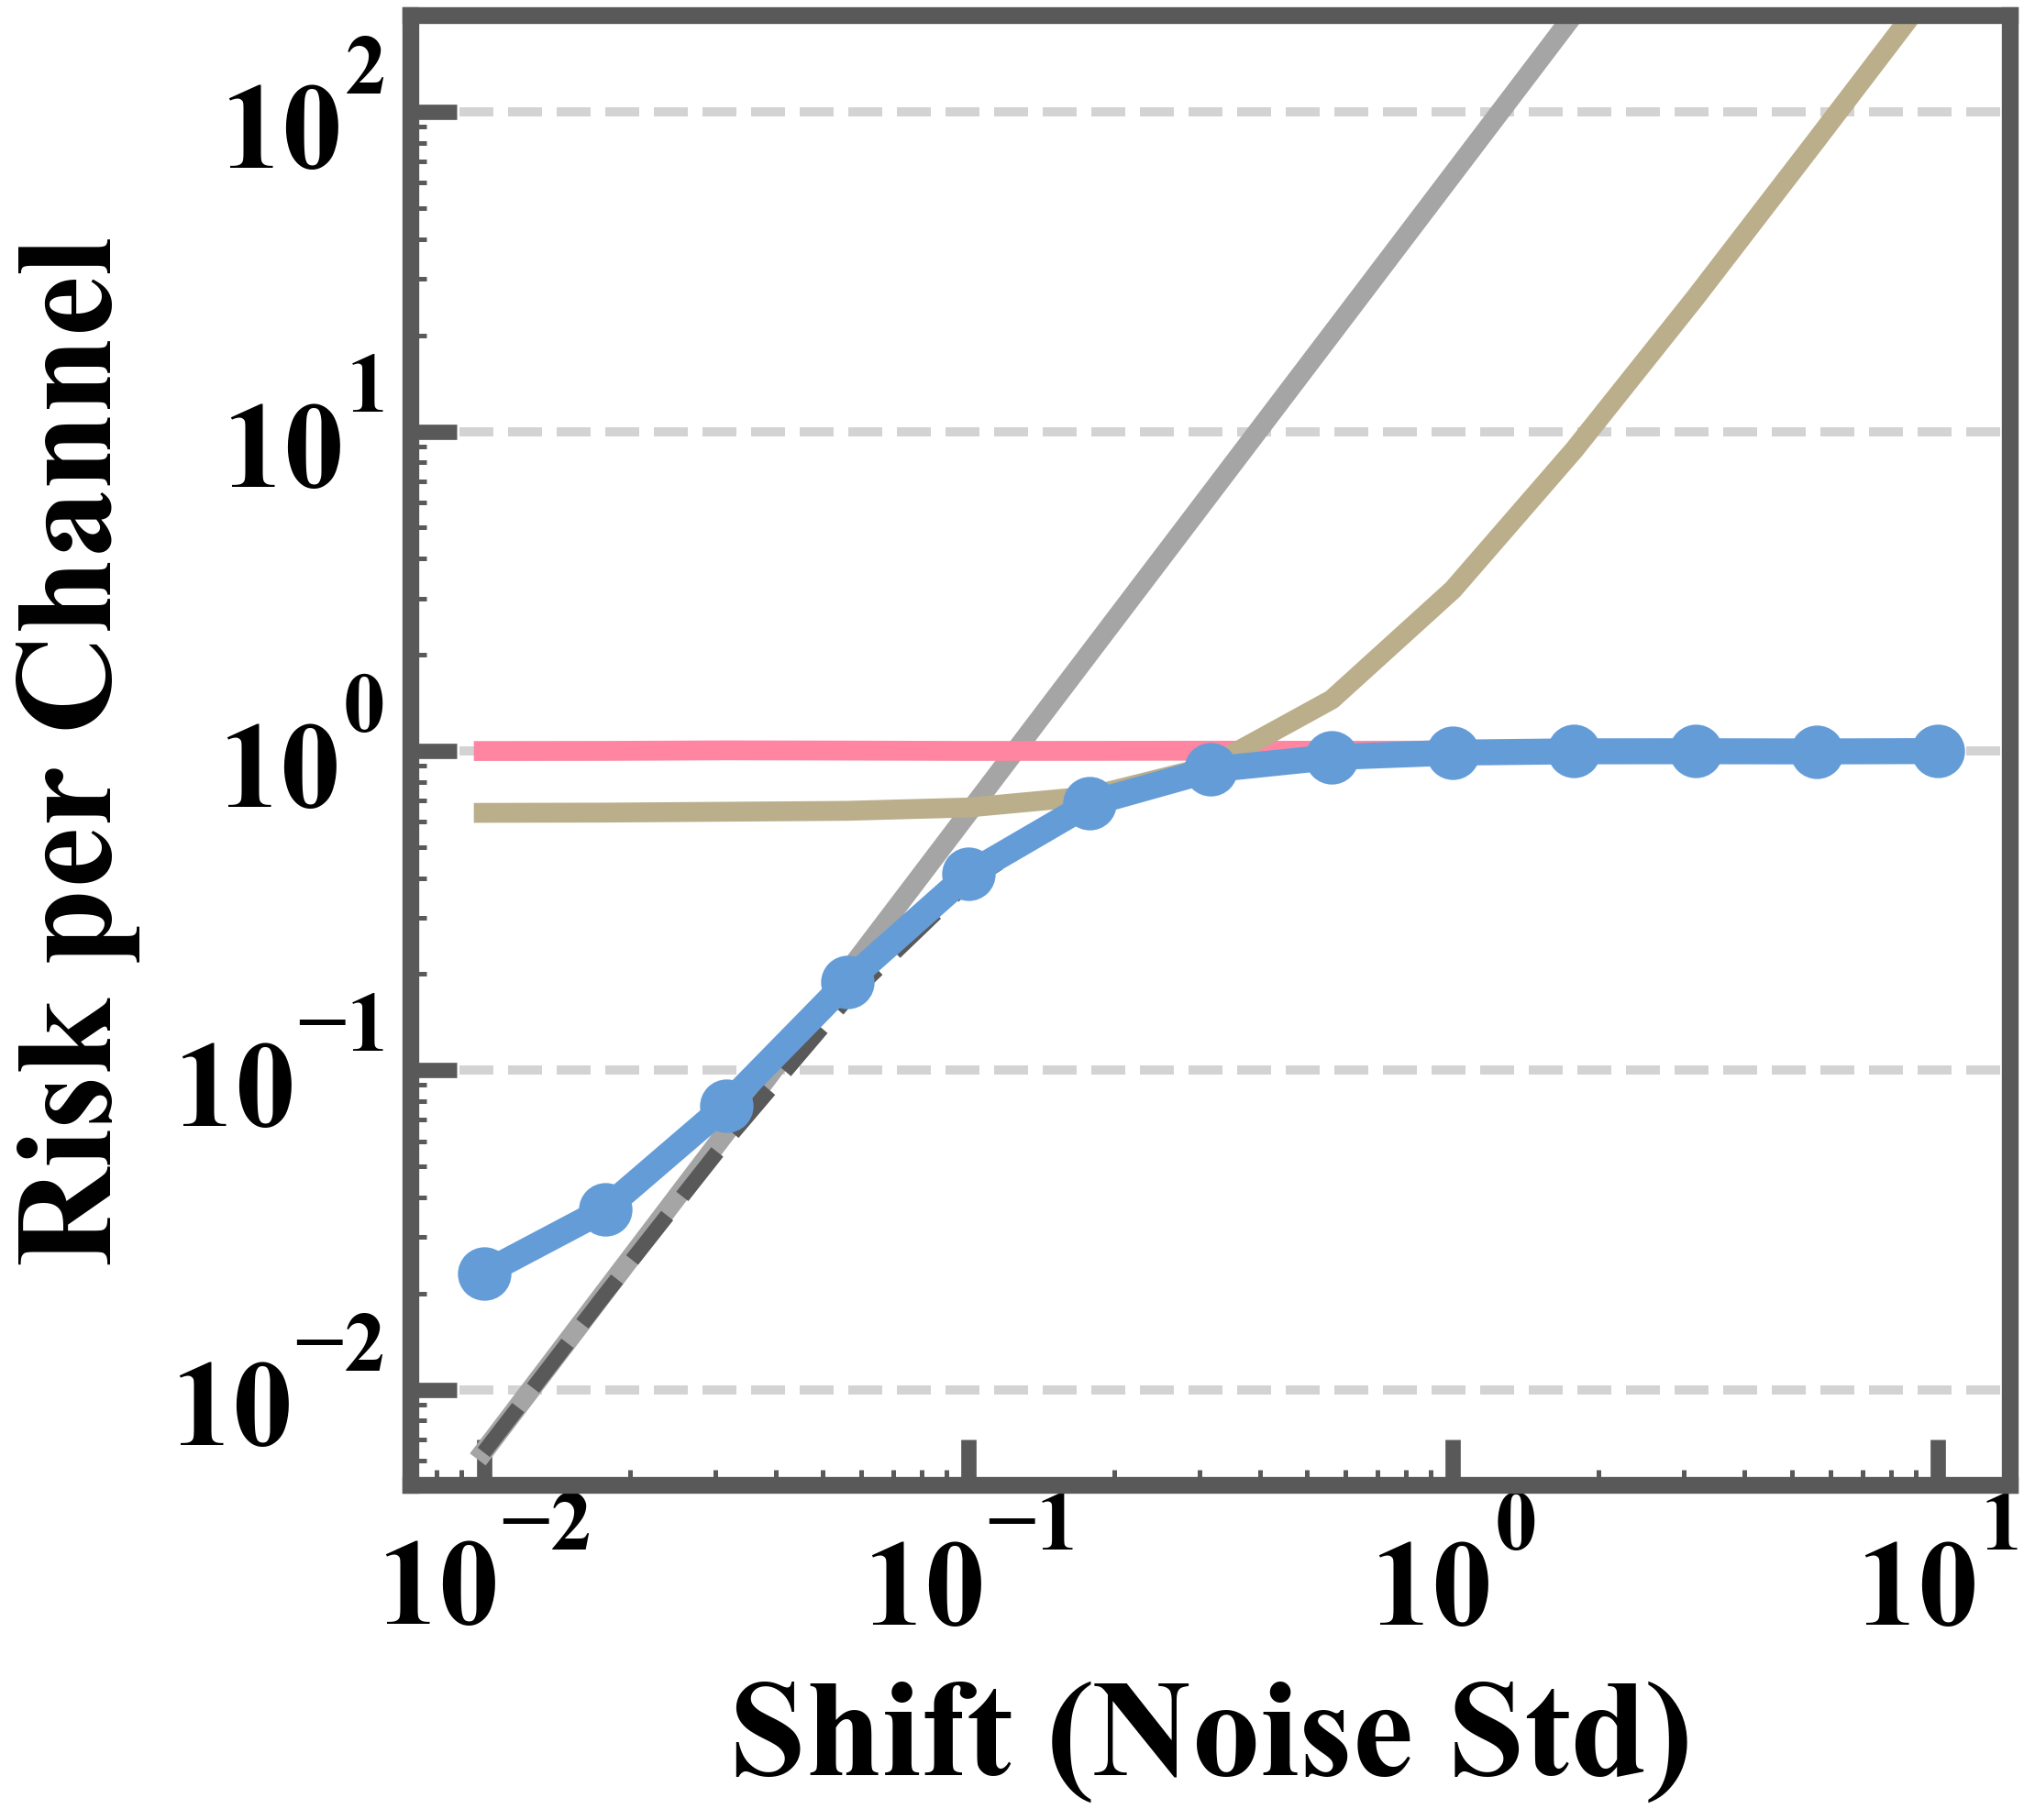
\includegraphics[width=\linewidth]{figures/exp/synthetic/risk_n64_gauss_s1p0.png}
        \caption{Gaussian, $n{=}64$.}
    \end{subfigure}
    \begin{subfigure}[t]{0.32\columnwidth}
        \centering
        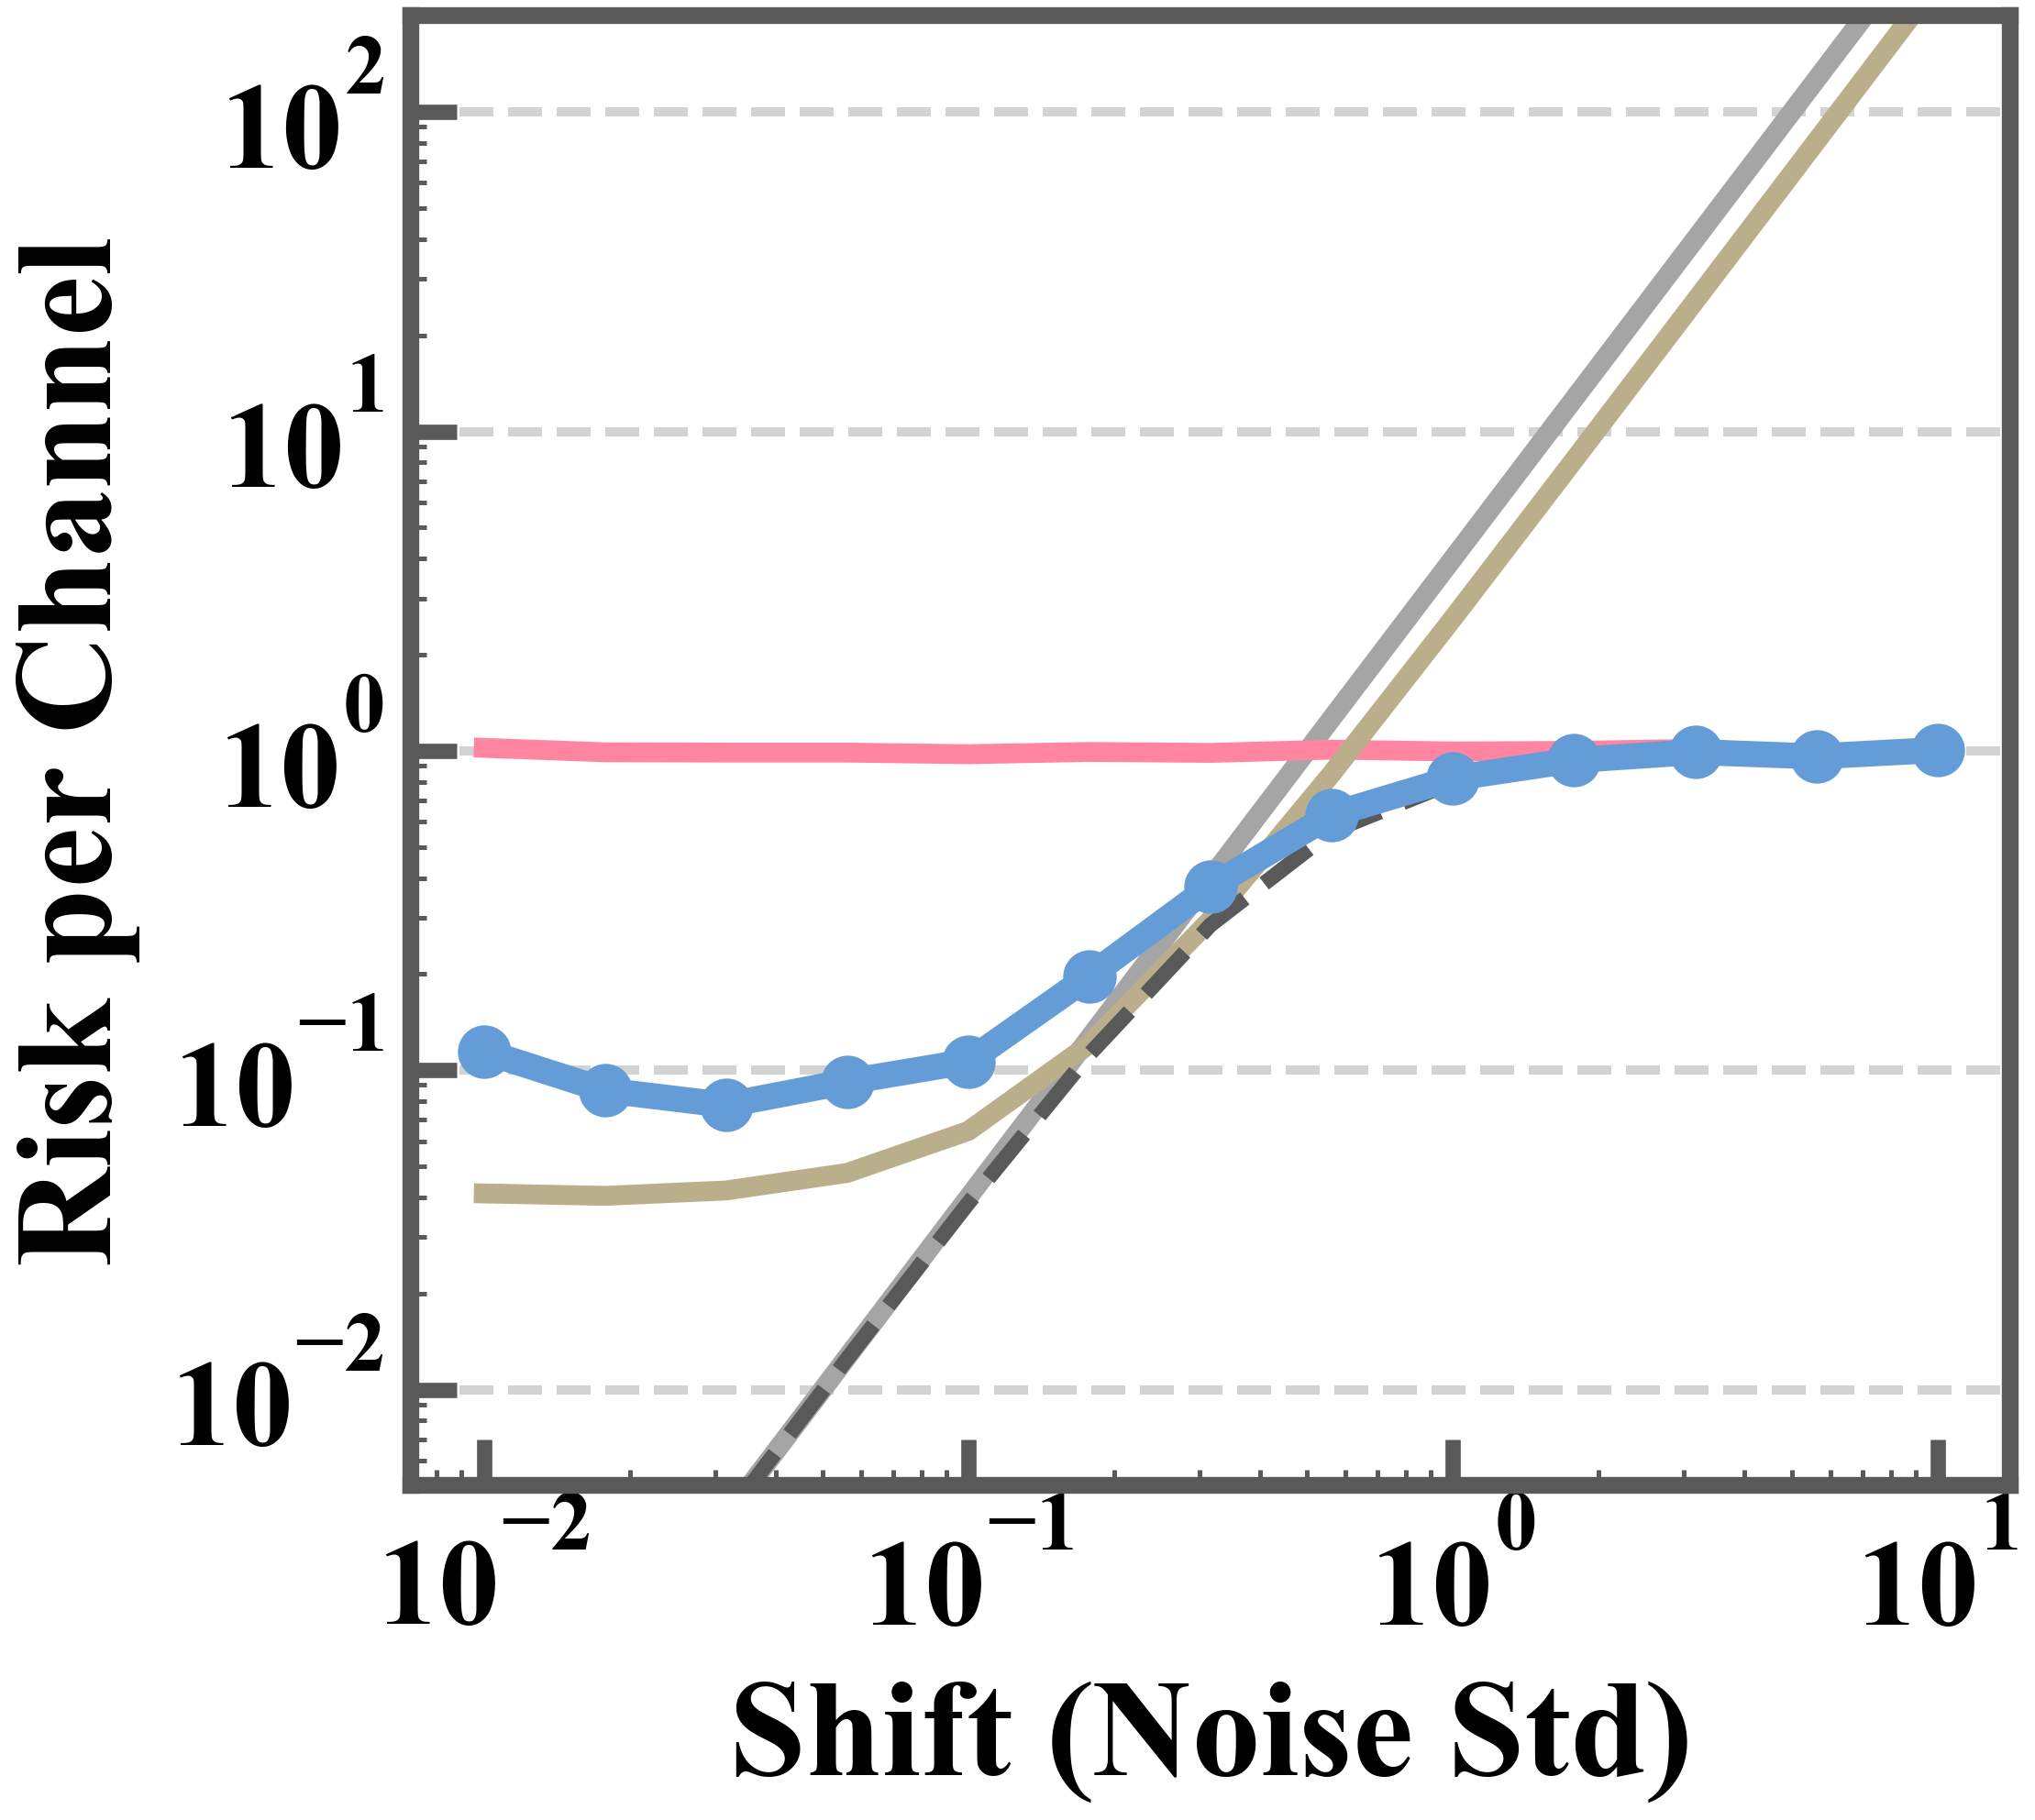
\includegraphics[width=\linewidth]{figures/exp/synthetic/risk_n4_student_t3_s1p0.png}
        \caption{Student-$t_3$, $n{=}4$.}
    \end{subfigure}\hfill
    \begin{subfigure}[t]{0.32\columnwidth}
        \centering
        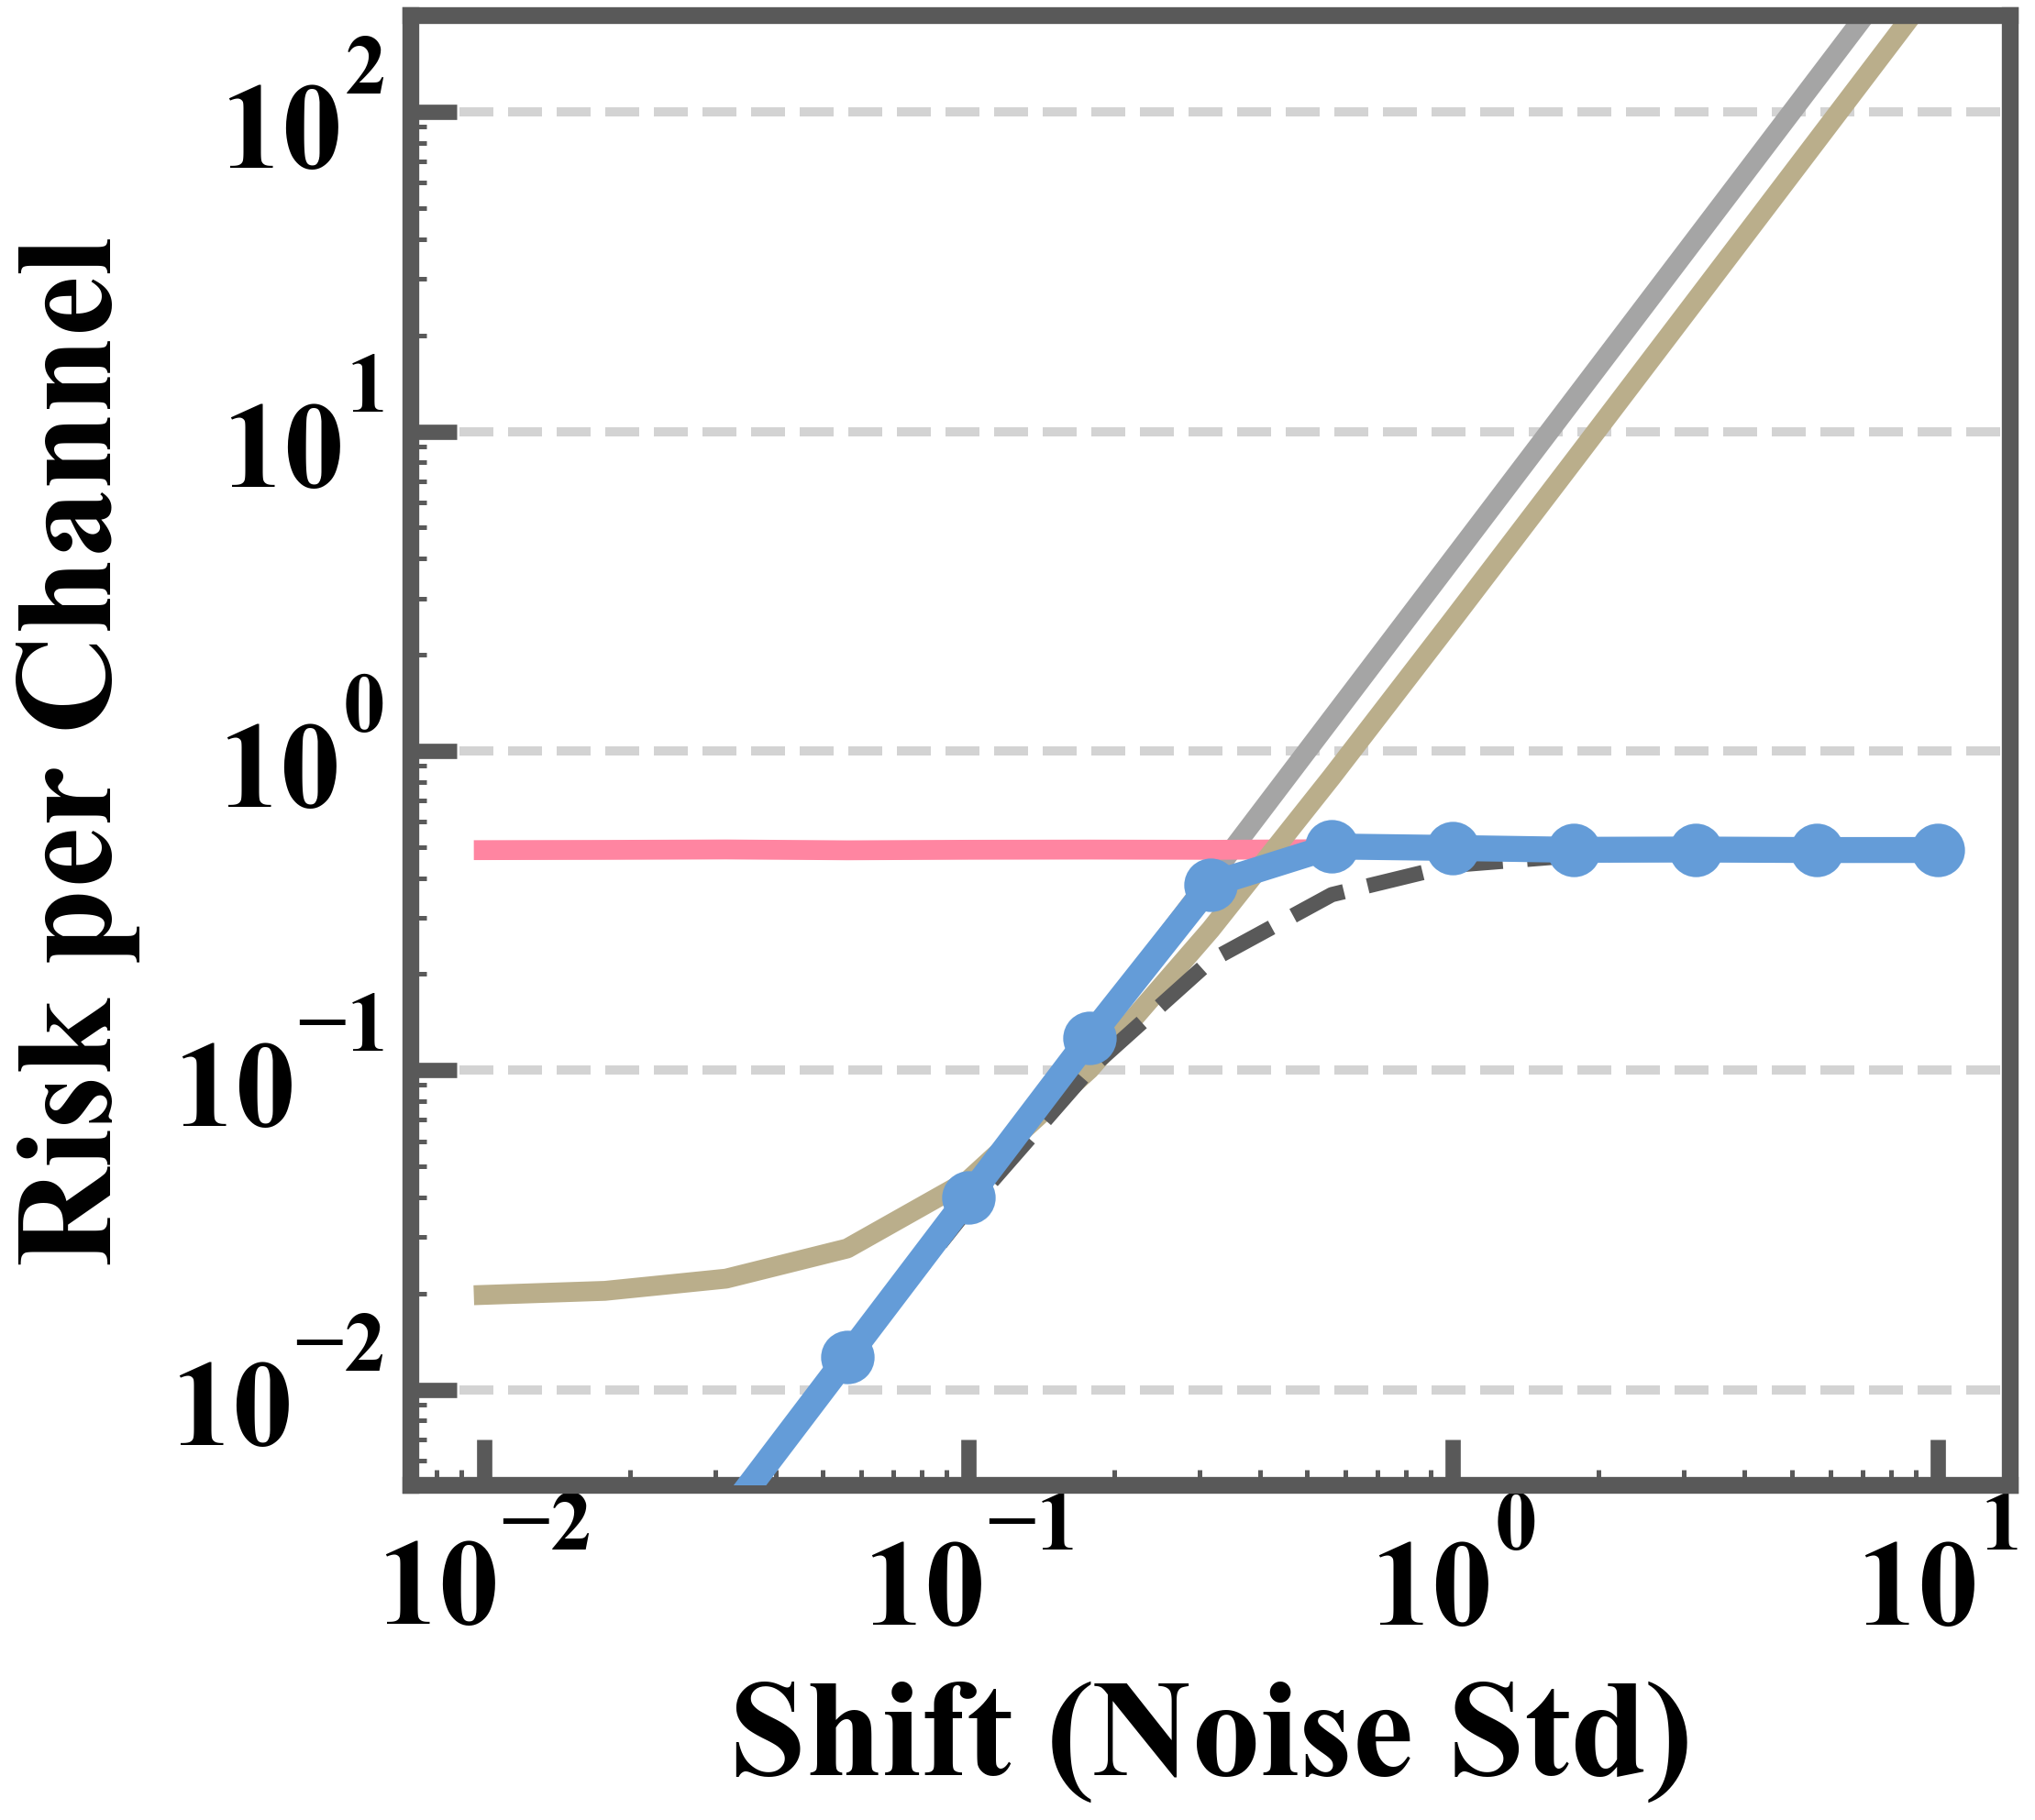
\includegraphics[width=\linewidth]{figures/exp/synthetic/risk_n4_gauss_s0p7.png}
        \caption{Noise $0.7\times$, $n{=}4$.}
    \end{subfigure}\hfill
    \begin{subfigure}[t]{0.32\columnwidth}
        \centering
        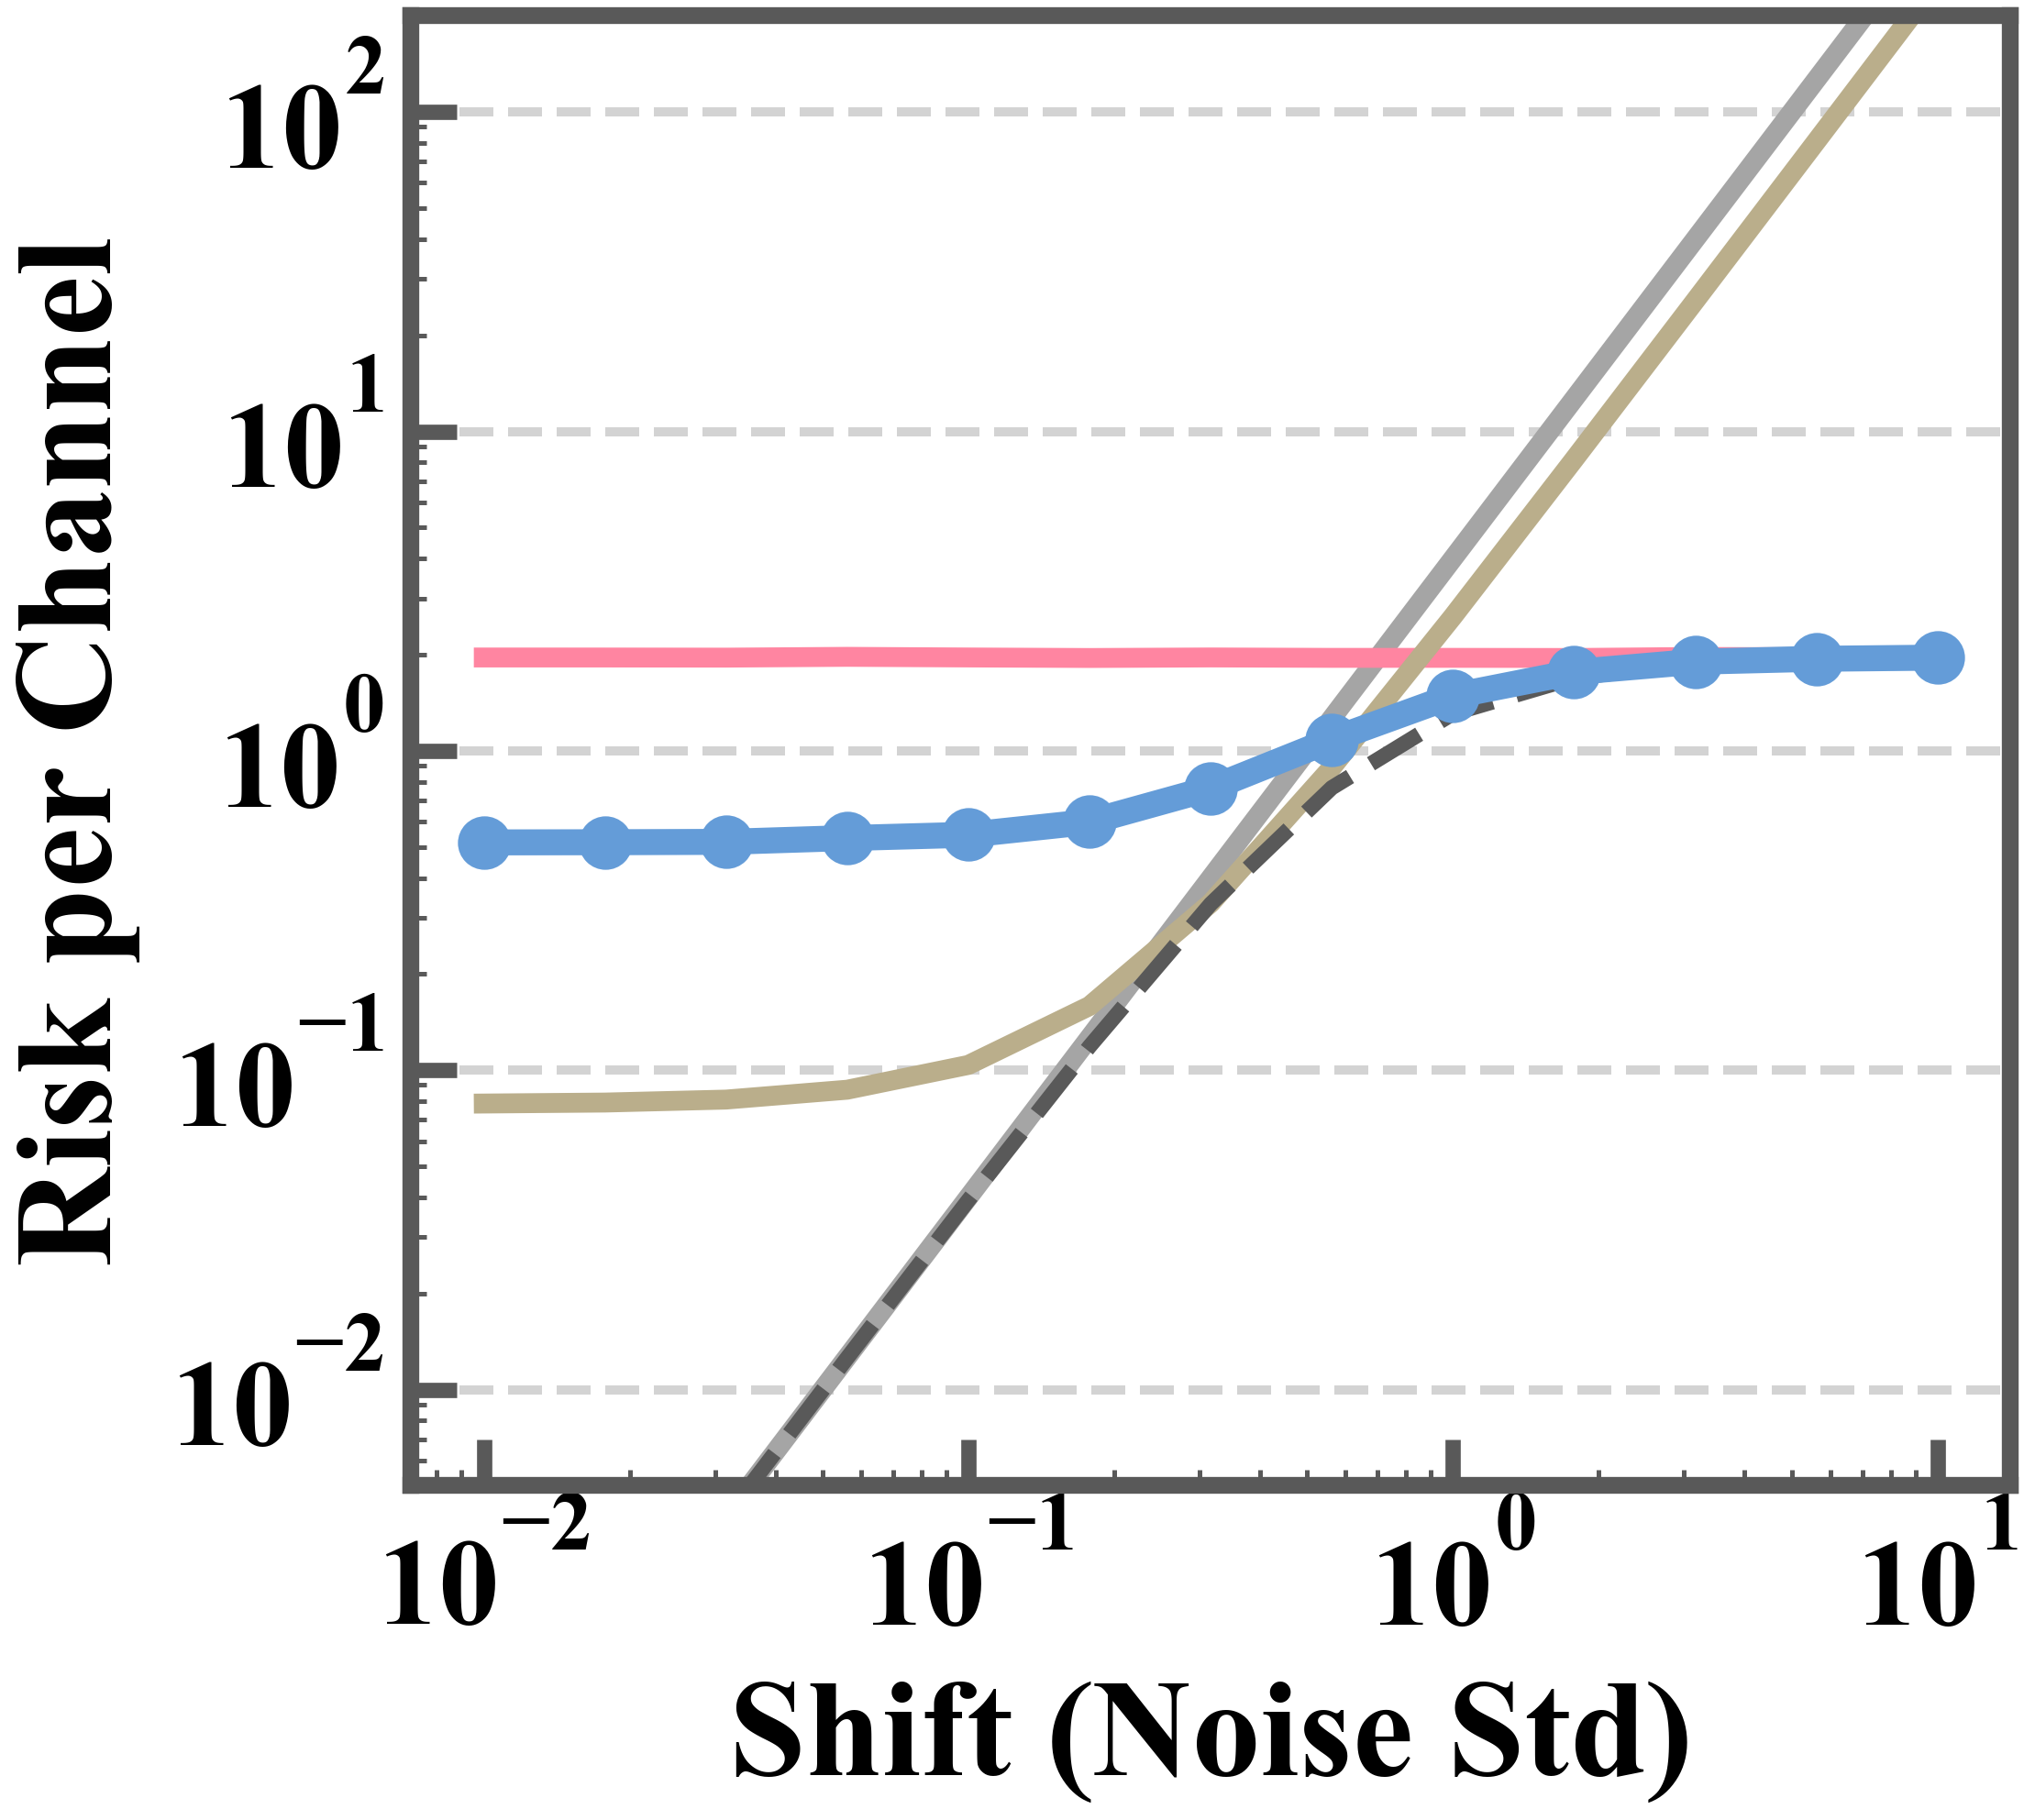
\includegraphics[width=\linewidth]{figures/exp/synthetic/risk_n4_gauss_s1p4.png}
        \caption{Noise $1.4\times$, $n{=}4$.}
    \end{subfigure}
    \caption{Risk per channel as a function of the per-channel shift in the simulation (log scales), with the legend of Figure~\ref{fig:teaser-figure}: Source (grey), TBN (pink), Prior-BN with $N{=}16$ (khaki), the oracle weight (dashed) and SourceStein (blue).}
    \label{fig:apdx-synthetic}
\end{figure}
